\documentclass[journal]{vgtc}                % final (journal style)
%\documentclass[review,journal]{vgtc}         % review (journal style)
%\documentclass[widereview]{vgtc}             % wide-spaced review
%\documentclass[preprint,journal]{vgtc}       % preprint (journal style)

%% Uncomment one of the lines above depending on where your paper is
%% in the conference process. ``review'' and ``widereview'' are for review
%% submission, ``preprint'' is for pre-publication, and the final version
%% doesn't use a specific qualifier.

%% Please use one of the ``review'' options in combination with the
%% assigned online id (see below) ONLY if your paper uses a double blind
%% review process. Some conferences, like IEEE Vis and InfoVis, have NOT
%% in the past.

%% Please note that the use of figures other than the optional teaser is not permitted on the first page
%% of the journal version.  Figures should begin on the second page and be
%% in CMYK or Grey scale format, otherwise, colour shifting may occur
%% during the printing process.  Papers submitted with figures other than the optional teaser on the
%% first page will be refused. Also, the teaser figure should only have the
%% width of the abstract as the template enforces it.

%% These few lines make a distinction between latex and pdflatex calls and they
%% bring in essential packages for graphics and font handling.
%% Note that due to the \DeclareGraphicsExtensions{} call it is no longer necessary
%% to provide the the path and extension of a graphics file:
%% 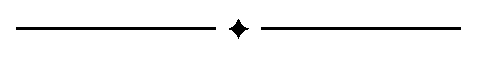
\includegraphics{diamondrule} is completely sufficient.
%%
\ifpdf%                                % if we use pdflatex
  \pdfoutput=1\relax                   % create PDFs from pdfLaTeX
  \pdfcompresslevel=9                  % PDF Compression
  \pdfoptionpdfminorversion=7          % create PDF 1.7
  \ExecuteOptions{pdftex}
  \usepackage{graphicx}                % allow us to embed graphics files
  \DeclareGraphicsExtensions{.pdf,.png,.jpg,.jpeg} % for pdflatex we expect .pdf, .png, or .jpg files
\else%                                 % else we use pure latex
  \ExecuteOptions{dvips}
  \usepackage{graphicx}                % allow us to embed graphics files
  \DeclareGraphicsExtensions{.eps}     % for pure latex we expect eps files
\fi%

%% it is recomended to use ``\autoref{sec:bla}'' instead of ``Fig.~\ref{sec:bla}''
\graphicspath{{figures/}{pictures/}{images/}{./}} % where to search for the images

\usepackage{microtype}                 % use micro-typography (slightly more compact, better to read)
\PassOptionsToPackage{warn}{textcomp}  % to address font issues with \textrightarrow
\usepackage{textcomp}                  % use better special symbols
\usepackage{mathptmx}                  % use matching math font
\usepackage{times}                     % we use Times as the main font
\renewcommand*\ttdefault{txtt}         % a nicer typewriter font
\usepackage{cite}                      % needed to automatically sort the references
\usepackage{tabu}                      % only used for the table example
\usepackage{booktabs}                  % only used for the table example
%% We encourage the use of mathptmx for consistent usage of times font
%% throughout the proceedings. However, if you encounter conflicts
%% with other math-related packages, you may want to disable it.

%% In preprint mode you may define your own headline.
%\preprinttext{To appear in IEEE Transactions on Visualization and Computer Graphics.}

%% If you are submitting a paper to a conference for review with a double
%% blind reviewing process, please replace the value ``0'' below with your
%% OnlineID. Otherwise, you may safely leave it at ``0''.
\onlineid{0}

%% declare the category of your paper, only shown in review mode
\vgtccategory{Research}
%% please declare the paper type of your paper to help reviewers, only shown in review mode
%% choices:
%% * algorithm/technique
%% * application/design study
%% * evaluation
%% * system
%% * theory/model
\vgtcpapertype{please specify}

%% Paper title.
\title{Global Illumination for Fun and Profit}

%% This is how authors are specified in the journal style

%% indicate IEEE Member or Student Member in form indicated below
\author{Roy G. Biv, Ed Grimley, \textit{Member, IEEE}, and Martha Stewart}
\authorfooter{
%% insert punctuation at end of each item
\item
 Roy G. Biv is with Starbucks Research. E-mail: roy.g.biv@aol.com.
\item
 Ed Grimley is with Grimley Widgets, Inc.. E-mail: ed.grimley@aol.com.
\item
 Martha Stewart is with Martha Stewart Enterprises at Microsoft
 Research. E-mail: martha.stewart@marthastewart.com.
}

%%%%%%%%%%%%%%%%%%%%%%%%%%%%%%%%%%%%%%%%%%%%%
\label{sec:abstract}
%%%%%%%%%%%%%%%%%%%%%%%%%%%%%%%%%%%%%%%%%%%%%
%% Abstract section.

\abstract{Understanding and debugging distributed systems is a
difficult task. Without proper tools developers are forced to inspect
logs from diverse machines. Tracing tools are used track distributed
executions based on control flow, and are typically accompanied by a
visualization front end for ease of use, and comprehension. Here we
propose a visualization for state based tracing. Our prior work used
t-SNE to visually cluster an execution. This approach took minutes on
traces of over 100 trace points, and over 300 variables, a significant
barrier to interactivity. In addition we used inferred data invariants
as a characterization of a systems properties. Lists of such
invariants totalled in the hundreds, and were incomprehensible to
users. Here we propose algorithmic, and architectural techniques for
improving the performance of t-SNE for the sake of interactivity, and
a novel technique for automatically extracting interesting data
invariants to reduce their cardinally, and increase
comprehensibility.}
%% end of abstract


%%%%%%%%%%%%%%%%%%%%%%%%%%%%%%%%%%%%%%%%%%%%%
\section{Introduction and Motivation}
\label{sec:intro}
%%%%%%%%%%%%%%%%%%%%%%%%%%%%%%%%%%%%%%%%%%%%%


The complexities of distributed systems have long plagued their
developers. Writing code which executes on various machines is
intrinsically more complicated due to networking eccentricities, such
as failures, partitions, and message delays. Debugging and checking
the correctness of such systems is laborious and technical, as
developers must inspect large logs for small discrepancies in expected
values, and timestamps. At scale auxiliary tools are necessary for
interpreting logs and making them understandable. Typically tracing tools
are used to reconstruct the communication of nodes throughout a
system, order their events, and present developers with a
comprehensive view of an execution.
%%
    Tracing tools alone still produce large amounts of data, albeit
    their structure is more understandable than raw logs. Typically
    tracing tools are equipped with a visual front end, allowing users
    to quickly observe the behaviour of executions, and under scrutiny
    identify irregular or bugging behaviour. No one tracing technique
    is sufficient for debugging distributed systems. While most tracing
    tools are concerned with debugging they typically fall into 3 sub
    categories of performance tuning, distributed control flow, and
    model checking. Each of these tracing objectives have different
    flavors of visualization which pair with them. We overview these
    visualization techniques in Section~\ref{sec:related}
%%

We propose a tracing tool which captures state similar to a model
checking trace tools, with the exception that rather than logging
control flow, our tracing tool only logs a distributed programs state.
Such tracing is unconventional and does not fit nicely into the
aforementioned tracing categories. As such our unique requirements
demand innovative visualization solutions. Entirely state based program
analysis has ties in the world of trajectory
programming~\cite{Waterland:2014:AAS:2654822.2541985,181250,Waterland:2013:CC:2485732.2485749}.
In trajectory analysis simple ML techniques such as weather man, and
mean prediction, as well as linear, and logistic regression are used
to automatically predict and parrallelize computation based solely on
state analysis.

Our proposed visualization for traces of program state applies a
similar ML technique, t-SNE clustering, a dimensionality reduction
algorithm~\cite{Hinton_visualizingdata}. We leverage t-SNE to clusters
points in a programs execution based on the similarities of a programs
state.  T-SNE requires a distancing function to cluster state, our
distance function is as follows. The distance between two trace points
$p$ and $p'$, whose state is composed of an identical set of variables
with potentially different values. For each matching pair of variables
XOR them together. Each 1 bit in the resultant XOR is a difference of
1 bit between the variables. We calculate the difference between two
variables as the number of one bits in the XOR. The distance between
trace points $p$ and $p'$ is the euclidean norm of all variable
distances.

We found the results of our initial technique promising, and the high level
behaviour of distributed programs we traced. However, our visualization suffers
due to a high level of computational complexity in running t-SNE. A single step
of the iterative t-SNE algorithm is $O(n)$, and the algorithm is typically
executed for greater that 20 iterations before a reasonable clustering is
obtained. Typical runtimes for traces consisting of 80 - 100 trace points,
containing 80 - 100 variables each resulted in runtimes in the tens of minutes.
This significant barrier to interactivity lead us to alter the architecture of
our tool, and implement parallel t-SNE to achieve interactive sub 10s
computation times. 

Our prototype visualization allowed users to inspect trace points, and
view individual variable values, without the ability to compare
points. All variables were weighted equally when computing weights.
Our interactivity goals are two fold first developers should be able
to query two points, and inspect variables which caused them to be
distant from one another. Second we acknowledge that all variables are
not of equal importance in a program. Some variables values
drastically alter the behaviour of a program while other do not. To
this end we extended our interface to support re-clustering with
increased weights for important user specified variables.

An additional feature of our tracing tool is the analysis of
distributed data invariants. We infer invariants using Dinv, a
distributed front end for Daikon~\cite{Ernst99dynamicallydiscovering}.
These invariants are inferred over entire traces of an execution, and
the number of invariants can be large and incomprehensible (300-400).
In addition to our improvements of t-SNE we refined our invariant
analysis by first, logically detecting t-SNE clusters using k-Means
clustering, deriving per cluster invariants, and refining those
further to unique invariants for each cluster. This processing step
greatly reduces spurious, and uninteresting invariants, and profiles
cluster behaviour more precisely.

The rest of the paper is laid out as follows.
Section~\ref{sec:related} covers related work. Section~\ref{sec:scope}
overviews the scope of our contributions, and Section~\ref{sec:imp}
covers our implementation. Section~\ref{sec:res} details our
performance results and data refinement accuracy. Finally
Section~\ref{sec:dafw} and Section~\ref{sec:conclusion} denote
potential future work, and the conclusion of the paper.

\section{Background}
\label{sec:background}


\noindent{\textbf{Distributed Snapshot}} is an algorithm which
proposes that consistent distributed state can be captured without
interfering with the execution of a system itself
~\cite{dist_snapshots_Chandy1985}.  Distributed snapshots can be
computed online or mined from a log containing vector clocks which
provide a partial ordering of events in a
system~\cite{mattern_vector_clocks_1989}. We consider distributed
snapshots to be a fundamental granularity for examining consistent
state. Our state analysis technique is therefore applied at the level
of a distributed snapshot.

\noindent{\textbf{\dinv}} is a tool which detects likely data
invariants in distributed systems~\cite{dinv}. \dinv operates by
instrumenting distributed systems to log system state and vector
clocks.  Execution logs from the nodes of the system are merged
together, and the state of the system is reconstructed and output as a
distributed system trace. \dinv leverages Daikon to automatically
infer data invariants on the trace.  We plan to use \dinv as a tool
for capturing distributed state.

\noindent{\textbf{Visualization}} is useful for helping users
comprehend complicated data.  Understanding distributed systems is a
challenging task for system designers, software developers and
students because of their inherent complexity.  Prior work on the
visualization on system traces has demonstrated that similarities in
the traces between software versions can be meaningfully conveyed to
developers~\cite{6613833}. Alternative work has demonstrated that
visualizing concurrent system traces using partial orderings can help
developers reason about interleaving
executions~\cite{6650534}~\cite{7272586}. We consider the state of a
system to be a direct artifact of a system trace. To our knowledge no
attempts have been made to visualize distributed system traces, and by
extension distributed state traces.

%There are a few studies focusing on 
%performance diagnositics of parallel or distributed systems, but few are done
%to understand the distributed nature in terms of state machines: 
%how distributed states transit.
%Visualization is suitable when there is enough data but no automatic algorithms
%to dig out the insights that people are looking for.  Here we can generate logs
%that we need by \textbf{TODO}, and there does not exist a general model that 
%can capture the distributed nature.

%\begin{itemize}
%\item modular visualization of distributed systems
%\item pip \textit{http://issg.cs.duke.edu/pip/}
%\item Overview: A Framework for Generic Online Visualization of Distributed
%Systems
%\item Jumpshot \textit{http://www.mcs.anl.gov/research/projects/perfvis/software/viewers/}
%\item vampire: http://citeseer.ist.psu.edu/viewdoc/summary?doi=10.1.1.38.1615
%\end{itemize}

\section{Proposed Approach}
\label{sec:proposed-approach}

Out goal is to visualize distributed state in a comprehensive way to
provide developers with an intuition about faulty behaviour. In order
to capture distributed state through variable logging, and the
aggregation of individual node state, we will leverage \dinv, a tool
for detecting likely data invariants in distributed
systems~\cite{dinv}.

Distributed state is inherently complex. In its raw form it consists
of partially ordered instances of variable values. This raw data is
classically hard to reason about. In order to convey distributed state
to a developer it must be summarized. We propose that the behaviour of
a distributed system under correct execution follows predicable
patters. Further that these patters are reflected the systems state.
The first contribution that our project seeks to make is a state
transition function $diff$ which measures the difference between
instances of distributed state. We recognize that many functions for
measuring state transitions could exist, our goal is to identify a
$diff$ function which is sensitive to state transitions, and is
normalized during repetitious behaviour.

Our initial approach will be to measure state transitions as the XOR
difference between variables in separate instances of distributed
state. We formalize the state $\sigma$ of a system to be a vector of
variables $V = {v_1,v_2,\dots,v_n}$. The XOR difference between two
states $\sigma_i$ and $\sigma_j$ is $XOR(V_i,V_j)$. The resulting
vector contains an indices for the XOR difference between each
variable. The vector itself is $n$ dimensional and represents the XOR
velocity of the systems state. To measure the effectiveness of our
$diff$ function, we will initially plot its output as a simple line
graph and check if predictable repetitions patters emerge between
executions.  Furthermore, we plan to plot the first and second order
derivatives of $diff$, $diff'$ and $diff''$ respectively to determine
if they also exhibit predictable patters. Initially we will try to
detect patterns in Ricart-Agrawala. If predictable patters emerge we
introduce a bug which causes the algorithm to violate mutual
exclusion. If predictable patterns emerge we will expand our research
into larger more general system. If the difference is not noticeable
but patterns emerge we will attempt to revise our visualization to
better reflect the property. If no alternative visualizations
demonstrate the irregularity, we will refine our $diff$ function to be
more specific to Ricart-Agrawala's state variables.

\section{Evaluation}
\label{sec:evaluation}

To evaluate \dviz we will conduct a user study in which participants will use
\dviz to identify buggy distributed systems. The purpose of the study will be
to demonstrate that \dviz's output is useful for detecting buggy executions.
Participants will be shown multiple visualization generated from the executions
of three systems. To demonstrate \dviz's generality the system will be composed
of a cross section of popular distributed applications. Specifically the
systems will be etcd Raft~\cite{etcdraft}, Groupcache~\cite{groupcache} and
Hashicorp Swim~\cite{das2002swim}.  In all cases bugs will be introduced into the
systems and the buggy visualization will be displayed alongside the non-faulty
executions. Etcd Raft will be modified so that leader elections will result in
more than one leader.  Groupcache will not adhere to its key ownership policy.
Swim will not fully propagate event messages to it's cluster. Study participants
will be given a brief description of the systems and will be asked to select the
visualization which they suspect to be faulty. Upon selecting a visualization
participants will be asked to identify which aspects of the visual prompted
their choice.  Finally, they will be shown snippets of source code from the
buggy execution, and be asked to identify the block of code responsible for the
irregular visualization.


\section{Timeline}
\label{sec:timeline}

\begin{itemize}
    \item \textbf{Sept 25 - Oct 15} Write and revise proposal
    \item \textbf{Oct 16 - 22} Implement Prototype
    \item \textbf{Oct 23 - Nov 5} Test on various systems and revise design
    \item \textbf{Nov 6 - 20} Collect results and organize user study
    \item \textbf{Nov 20 - Dec 4} Perform user study
    \item \textbf{Dec 5 - 15} Write project report and prepare presentation
    \item \textbf{TBD} Present project and submit report
\end{itemize}

%other entries to be set up for journal
\shortauthortitle{Biv \MakeLowercase{\textit{et al.}}: Global Illumination for Fun and Profit}
%\shortauthortitle{Firstauthor \MakeLowercase{\textit{et al.}}: Paper Title}

%% Abstract section.
\abstract{Duis autem vel eum iriure dolor in hendrerit in vulputate
velit esse molestie consequat, vel illum dolore eu feugiat nulla
facilisis at vero eros et accumsan et iusto odio dignissim qui blandit
praesent luptatum zzril delenit augue duis dolore te feugait nulla
facilisi. Lorem ipsum dolor sit amet, consectetuer adipiscing elit,
sed diam nonummy nibh euismod tincidunt ut laoreet dolore magna
aliquam erat volutpat. Ut wisi enim ad minim veniam, quis nostrud exerci tation ullamcorper
suscipit lobortis nisl ut aliquip ex ea commodo consequat. Duis autem
vel eum iriure dolor in hendrerit in vulputate velit esse molestie
consequat, vel illum dolore eu feugiat nulla facilisis at vero eros et
accumsan et iusto odio dignissim qui blandit praesent luptatum zzril
delenit augue duis dolore te feugait nulla facilisi.%
} % end of abstract

%% Keywords that describe your work. Will show as 'Index Terms' in journal
%% please capitalize first letter and insert punctuation after last keyword
\keywords{Radiosity, global illumination, constant time}

%% ACM Computing Classification System (CCS). 
%% See <http://www.acm.org/class/1998/> for details.
%% The ``\CCScat'' command takes four arguments.

\CCScatlist{ % not used in journal version
 \CCScat{K.6.1}{Management of Computing and Information Systems}%
{Project and People Management}{Life Cycle};
 \CCScat{K.7.m}{The Computing Profession}{Miscellaneous}{Ethics}
}

%% Uncomment below to include a teaser figure.
\teaser{
  \centering
  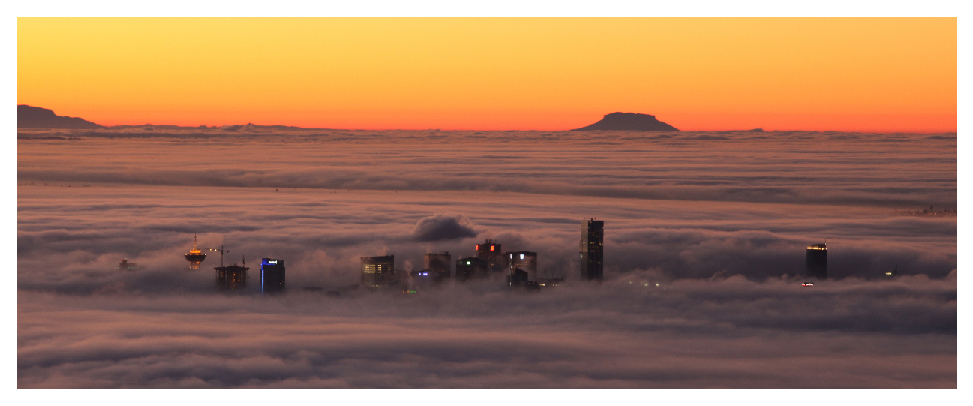
\includegraphics[width=\linewidth]{CypressView}
  \caption{In the Clouds: Vancouver from Cypress Mountain. Note that the teaser may not be wider than the abstract block.}
	\label{fig:teaser}
}

%% Uncomment below to disable the manuscript note
%\renewcommand{\manuscriptnotetxt}{}

%% Copyright space is enabled by default as required by guidelines.
%% It is disabled by the 'review' option or via the following command:
% \nocopyrightspace

\vgtcinsertpkg

%%%%%%%%%%%%%%%%%%%%%%%%%%%%%%%%%%%%%%%%%%%%%%%%%%%%%%%%%%%%%%%%
%%%%%%%%%%%%%%%%%%%%%% START OF THE PAPER %%%%%%%%%%%%%%%%%%%%%%
%%%%%%%%%%%%%%%%%%%%%%%%%%%%%%%%%%%%%%%%%%%%%%%%%%%%%%%%%%%%%%%%%

\begin{document}

%% The ``\maketitle'' command must be the first command after the
%% ``\begin{document}'' command. It prepares and prints the title block.

%% the only exception to this rule is the \firstsection command
\firstsection{Introduction}

\maketitle

%% \section{Introduction} %for journal use above \firstsection{..} instead
This template is for papers of VGTC-sponsored conferences such as IEEE VIS, IEEE VR, and ISMAR which are published as special issues of TVCG. The template does not contain the respective dates of the conference/journal issue, these will be entered by IEEE as part of the publication production process.

\section{Using the Style Template}

\begin{itemize}
\item Note that each author needs to have a separate entry in author footer on the bottom-left corner of the first page, merging two people (even if from the same institution) is not permitted.
\item The style uses the hyperref package, thus turns references into internal links. We thus recommend to make use of the ``\texttt{\textbackslash autoref\{reference\}}'' call (instead of ``\texttt{Figure\~{}\textbackslash ref\{reference\}}'' or similar) since ``\texttt{\textbackslash autoref\{reference\}}'' turns the entire reference into an internal link, not just the number. Examples: \autoref{fig:sample} and \autoref{tab:vis_papers}.
\item The style automatically looks for image files with the correct extension (eps for regular \LaTeX; pdf, png, and jpg for pdf\LaTeX), in a set of given subfolders (figures/, pictures/, images/). It is thus sufficient to use ``\texttt{\textbackslash includegraphics\{CypressView\}}'' (instead of ``\texttt{\textbackslash includegraphics\{pictures/CypressView.jpg\}}'').
\item For adding hyperlinks and DOIs to the list of references, you can use ``\texttt{\textbackslash bibliographystyle\{abbrv-doi-hyperref-narrow\}}'' (instead of ``\texttt{\textbackslash bibliographystyle\{abbrv\}}''). It uses the doi and url fields in a bib\TeX\ entry and turns the entire reference into a link, giving priority to the doi. The doi can be entered with or without the ``\texttt{http://dx.doi.org/}'' url part. See the examples in the bib\TeX\ file and the bibliography at the end of this template.\\[1em]
\textbf{Note 1:} occasionally (for some \LaTeX\ distributions) this hyper-linked bib\TeX\ style may lead to \textbf{compilation errors} (``\texttt{pdfendlink ended up in different nesting level ...}'') if a reference entry is broken across two pages (due to a bug in hyperref). In this case make sure you have the latest version of the hyperref package (i.\,e., update your \LaTeX\ installation/packages) or, alternatively, revert back to ``\texttt{\textbackslash bibliographystyle\{abbrv-doi-narrow\}}'' (at the expense of removing hyperlinks from the bibliography) and try ``\texttt{\textbackslash bibliographystyle\{abbrv-doi-hyperref-narrow\}}'' again after some more editing.\\[1em]
\textbf{Note 2:} the ``\texttt{-narrow}'' versions of the bibliography style use the font ``PTSansNarrow-TLF'' for typesetting the DOIs in a compact way. This font needs to be available on your \LaTeX\ system. It is part of the \href{https://www.ctan.org/pkg/paratype}{``paratype'' package}, and many distributions (such as MikTeX) have it automatically installed. If you do not have this package yet and want to use a ``\texttt{-narrow}'' bibliography style then use your \LaTeX\ system's package installer to add it. If this is not possible you can also revert to the respective bibliography styles without the ``\texttt{-narrow}'' in the file name.\\[1em]
DVI-based processes to compile the template apparently cannot handle the different font so, by default, the template file uses the \texttt{abbrv-doi} bibliography style but the compiled PDF shows you the effect of the \texttt{abbrv-doi-hyperref-narrow} style.
\end{itemize}

\section{Bibliography Instructions}

\begin{itemize}
\item Sort all bibliographic entries alphabetically but the last name of the first author. This \LaTeX/bib\TeX\ template takes care of this sorting automatically.
\item Merge multiple references into one; e.\,g., use \cite{Max:1995:OMF,Kitware:2003} (not \cite{Kitware:2003}\cite{Max:1995:OMF}). Within each set of multiple references, the references should be sorted in ascending order. This \LaTeX/bib\TeX\ template takes care of both the merging and the sorting automatically.
\item Verify all data obtained from digital libraries, even ACM's DL and IEEE Xplore  etc.\ are sometimes wrong or incomplete.
\item Do not trust bibliographic data from other services such as Mendeley.com, Google Scholar, or similar; these are even more likely to be incorrect or incomplete.
\item Articles in journal---items to include:
  \begin{itemize}
  \item author names
	\item title
	\item journal name
	\item year
	\item volume
	\item number
	\item month of publication as variable name (i.\,e., \{jan\} for January, etc.; month ranges using \{jan \#\{/\}\# feb\} or \{jan \#\{-{}-\}\# feb\})
  \end{itemize}
\item use journal names in proper style: correct: ``IEEE Transactions on Visualization and Computer Graphics'', incorrect: ``Visualization and Computer Graphics, IEEE Transactions on''
\item Papers in proceedings---items to include:
  \begin{itemize}
  \item author names
	\item title
	\item abbreviated proceedings name: e.\,g., ``Proc.\textbackslash{} CONF\_ACRONYNM'' without the year; example: ``Proc.\textbackslash{} CHI'', ``Proc.\textbackslash{} 3DUI'', ``Proc.\textbackslash{} Eurographics'', ``Proc.\textbackslash{} EuroVis''
	\item year
	\item publisher
	\item town with country of publisher (the town can be abbreviated for well-known towns such as New York or Berlin)
  \end{itemize}
\item article/paper title convention: refrain from using curly brackets, except for acronyms/proper names/words following dashes/question marks etc.; example:
\begin{itemize}
	\item paper ``Marching Cubes: A High Resolution 3D Surface Construction Algorithm''
	\item should be entered as ``\{M\}arching \{C\}ubes: A High Resolution \{3D\} Surface Construction Algorithm'' or  ``\{M\}arching \{C\}ubes: A high resolution \{3D\} surface construction algorithm''
	\item will be typeset as ``Marching Cubes: A high resolution 3D surface construction algorithm''
\end{itemize}
\item for all entries
\begin{itemize}
	\item DOI can be entered in the DOI field as plain DOI number or as DOI url; alternative: a url in the URL field
	\item provide full page ranges AA-{}-BB
\end{itemize}
\item when citing references, do not use the reference as a sentence object; e.\,g., wrong: ``In \cite{Lorensen:1987:MCA} the authors describe \dots'', correct: ``Lorensen and Cline \cite{Lorensen:1987:MCA} describe \dots''
\end{itemize}

\section{Example Section}

Lorem ipsum dolor sit amet, consetetur sadipscing elitr, sed diam
nonumy eirmod tempor invidunt ut labore et dolore magna aliquyam erat,
sed diam voluptua. At vero eos et accusam et justo duo dolores et ea
rebum. Stet clita kasd gubergren, no sea takimata sanctus est Lorem
ipsum dolor sit amet. Lorem ipsum dolor sit amet, consetetur
sadipscing elitr, sed diam nonumy eirmod tempor invidunt ut labore et
dolore magna aliquyam erat, sed diam
voluptua~\cite{Kitware:2003,Max:1995:OMF}. At vero eos et accusam et
justo duo dolores et ea rebum. Stet clita kasd gubergren, no sea
takimata sanctus est Lorem ipsum dolor sit amet. Lorem ipsum dolor sit
amet, consetetur sadipscing elitr, sed diam nonumy eirmod tempor
invidunt ut labore et dolore magna aliquyam erat, sed diam
voluptua. At vero eos et accusam et justo duo dolores et ea
rebum. Stet clita kasd gubergren, no sea takimata sanctus est.

\section{Exposition}

Duis autem vel eum iriure dolor in hendrerit in vulputate velit esse
molestie consequat, vel illum dolore eu feugiat nulla facilisis at
vero eros et accumsan et iusto odio dignissim qui blandit praesent
luptatum zzril delenit augue duis dolore te feugait nulla
facilisi. Lorem ipsum dolor sit amet, consectetuer adipiscing elit,
sed diam nonummy nibh euismod tincidunt ut laoreet dolore magna
aliquam erat volutpat~\cite{Kindlmann:1999:SAG}.

\begin{equation}
\sum_{j=1}^{z} j = \frac{z(z+1)}{2}
\end{equation}

Lorem ipsum dolor sit amet, consetetur sadipscing elitr, sed diam
nonumy eirmod tempor invidunt ut labore et dolore magna aliquyam erat,
sed diam voluptua. At vero eos et accusam et justo duo dolores et ea
rebum. Stet clita kasd gubergren, no sea takimata sanctus est Lorem
ipsum dolor sit amet. Lorem ipsum dolor sit amet, consetetur
sadipscing elitr, sed diam nonumy eirmod tempor invidunt ut labore et
dolore magna aliquyam erat, sed diam voluptua. At vero eos et accusam
et justo duo dolores et ea rebum. Stet clita kasd gubergren, no sea
takimata sanctus est Lorem ipsum dolor sit amet.

\subsection{Lorem ipsum}

Lorem ipsum dolor sit amet (see \autoref{tab:vis_papers}), consetetur sadipscing elitr, sed diam
nonumy eirmod tempor invidunt ut labore et dolore magna aliquyam erat,
sed diam voluptua. At vero eos et accusam et justo duo dolores et ea
rebum. Stet clita kasd gubergren, no sea takimata sanctus est Lorem
ipsum dolor sit amet. Lorem ipsum dolor sit amet, consetetur
sadipscing elitr, sed diam nonumy eirmod tempor invidunt ut labore et
dolore magna aliquyam erat, sed diam voluptua. At vero eos et accusam
et justo duo dolores et ea rebum. Stet clita kasd gubergren, no sea
takimata sanctus est Lorem ipsum dolor sit amet. Lorem ipsum dolor sit
amet, consetetur sadipscing elitr, sed diam nonumy eirmod tempor
invidunt ut labore et dolore magna aliquyam erat, sed diam
voluptua. At vero eos et accusam et justo duo dolores et ea
rebum. 

\begin{table}[tb]
  \caption{VIS/VisWeek accepted/presented papers: 1990--2015.}
  \label{tab:vis_papers}
  \scriptsize%
	\centering%
  \begin{tabu}{%
	r%
	*{7}{c}%
	*{2}{r}%
	}
  \toprule
   year & \rotatebox{90}{Vis/SciVis} &   \rotatebox{90}{SciVis conf} &   \rotatebox{90}{InfoVis} &   \rotatebox{90}{VAST} &   \rotatebox{90}{VAST conf} &   \rotatebox{90}{TVCG @ VIS} &   \rotatebox{90}{CG\&A @ VIS} &   \rotatebox{90}{VIS/VisWeek} \rotatebox{90}{incl. TVCG/CG\&A}   &   \rotatebox{90}{VIS/VisWeek} \rotatebox{90}{w/o TVCG/CG\&A}   \\
  \midrule
  2015 & 33 & 9 & 38 & 33 & 14 & 17 & 15 & 159 & 127 \\
  2014 & 34 &   & 45 & 33 & 21 & 20 &   & 153 & 133 \\
  2013 & 31 &   & 38 & 32 &   & 20 &   & 121 & 101 \\
  2012 & 42 &   & 44 & 30 &   & 23 &   & 139 & 116 \\
  2011 & 49 &   & 44 & 26 &   & 20 &   & 139 & 119 \\
  2010 & 48 &   & 35 & 26 &   &   &   & 109 & 109 \\
  2009 & 54 &   & 37 & 26 &   &   &   & 117 & 117 \\
  2008 & 50 &   & 28 & 21 &   &   &   & 99 & 99 \\
  2007 & 56 &   & 27 & 24 &   &   &   & 107 & 107 \\
  2006 & 63 &   & 24 & 26 &   &   &   & 113 & 113 \\
  2005 & 88 &   & 31 &   &   &   &   & 119 & 119 \\
  2004 & 70 &   & 27 &   &   &   &   & 97 & 97 \\
  2003 & 74 &   & 29 &   &   &   &   & 103 & 103 \\
  2002 & 78 &   & 23 &   &   &   &   & 101 & 101 \\
  2001 & 74 &   & 22 &   &   &   &   & 96 & 96 \\
  2000 & 73 &   & 20 &   &   &   &   & 93 & 93 \\
  1999 & 69 &   & 19 &   &   &   &   & 88 & 88 \\
  1998 & 72 &   & 18 &   &   &   &   & 90 & 90 \\
  1997 & 72 &   & 16 &   &   &   &   & 88 & 88 \\
  1996 & 65 &   & 12 &   &   &   &   & 77 & 77 \\
  1995 & 56 &   & 18 &   &   &   &   & 74 & 74 \\
  1994 & 53 &   &   &   &   &   &   & 53 & 53 \\
  1993 & 55 &   &   &   &   &   &   & 55 & 55 \\
  1992 & 53 &   &   &   &   &   &   & 53 & 53 \\
  1991 & 50 &   &   &   &   &   &   & 50 & 50 \\
  1990 & 53 &   &   &   &   &   &   & 53 & 53 \\
  \midrule
  \textbf{sum} & \textbf{1515} & \textbf{9} & \textbf{595} & \textbf{277} & \textbf{35} & \textbf{100} & \textbf{15} & \textbf{2546} & \textbf{2431} \\
  \bottomrule
  \end{tabu}%
\end{table}

\subsection{Mezcal Head}

Lorem ipsum dolor sit amet (see \autoref{fig:sample}), consetetur sadipscing elitr, sed diam
nonumy eirmod tempor invidunt ut labore et dolore magna aliquyam erat,
sed diam voluptua. At vero eos et accusam et justo duo dolores et ea
rebum. Stet clita kasd gubergren, no sea takimata sanctus est Lorem
ipsum dolor sit amet. Lorem ipsum dolor sit amet, consetetur
sadipscing elitr, sed diam nonumy eirmod tempor invidunt ut labore et
dolore magna aliquyam erat, sed diam voluptua. At vero eos et accusam
et justo duo dolores et ea rebum. Stet clita kasd gubergren, no sea
takimata sanctus est Lorem ipsum dolor sit amet. 

\subsubsection{Duis Autem}

Lorem ipsum dolor sit amet, consetetur sadipscing elitr, sed diam
nonumy eirmod tempor invidunt ut labore et dolore magna aliquyam erat,
sed diam voluptua. At vero eos et accusam et justo duo dolores et ea
rebum. Stet clita kasd gubergren, no sea takimata sanctus est Lorem
ipsum dolor sit amet. Lorem ipsum dolor sit amet, consetetur
sadipscing elitr, sed diam nonumy eirmod tempor invidunt ut labore et
dolore magna aliquyam erat, sed diam voluptua. At vero eos et accusam
et justo duo dolores et ea rebum. Stet clita kasd gubergren, no sea
takimata sanctus est Lorem ipsum dolor sit amet. Lorem ipsum dolor sit
amet, consetetur sadipscing elitr, sed diam nonumy eirmod tempor
invidunt ut labore et dolore magna aliquyam erat, sed diam
voluptua. At vero eos et accusam et justo duo dolores et ea
rebum. Stet clita kasd gubergren, no sea takimata sanctus est. Lorem
ipsum dolor sit amet.

\begin{figure}[tb]
 \centering % avoid the use of \begin{center}...\end{center} and use \centering instead (more compact)
 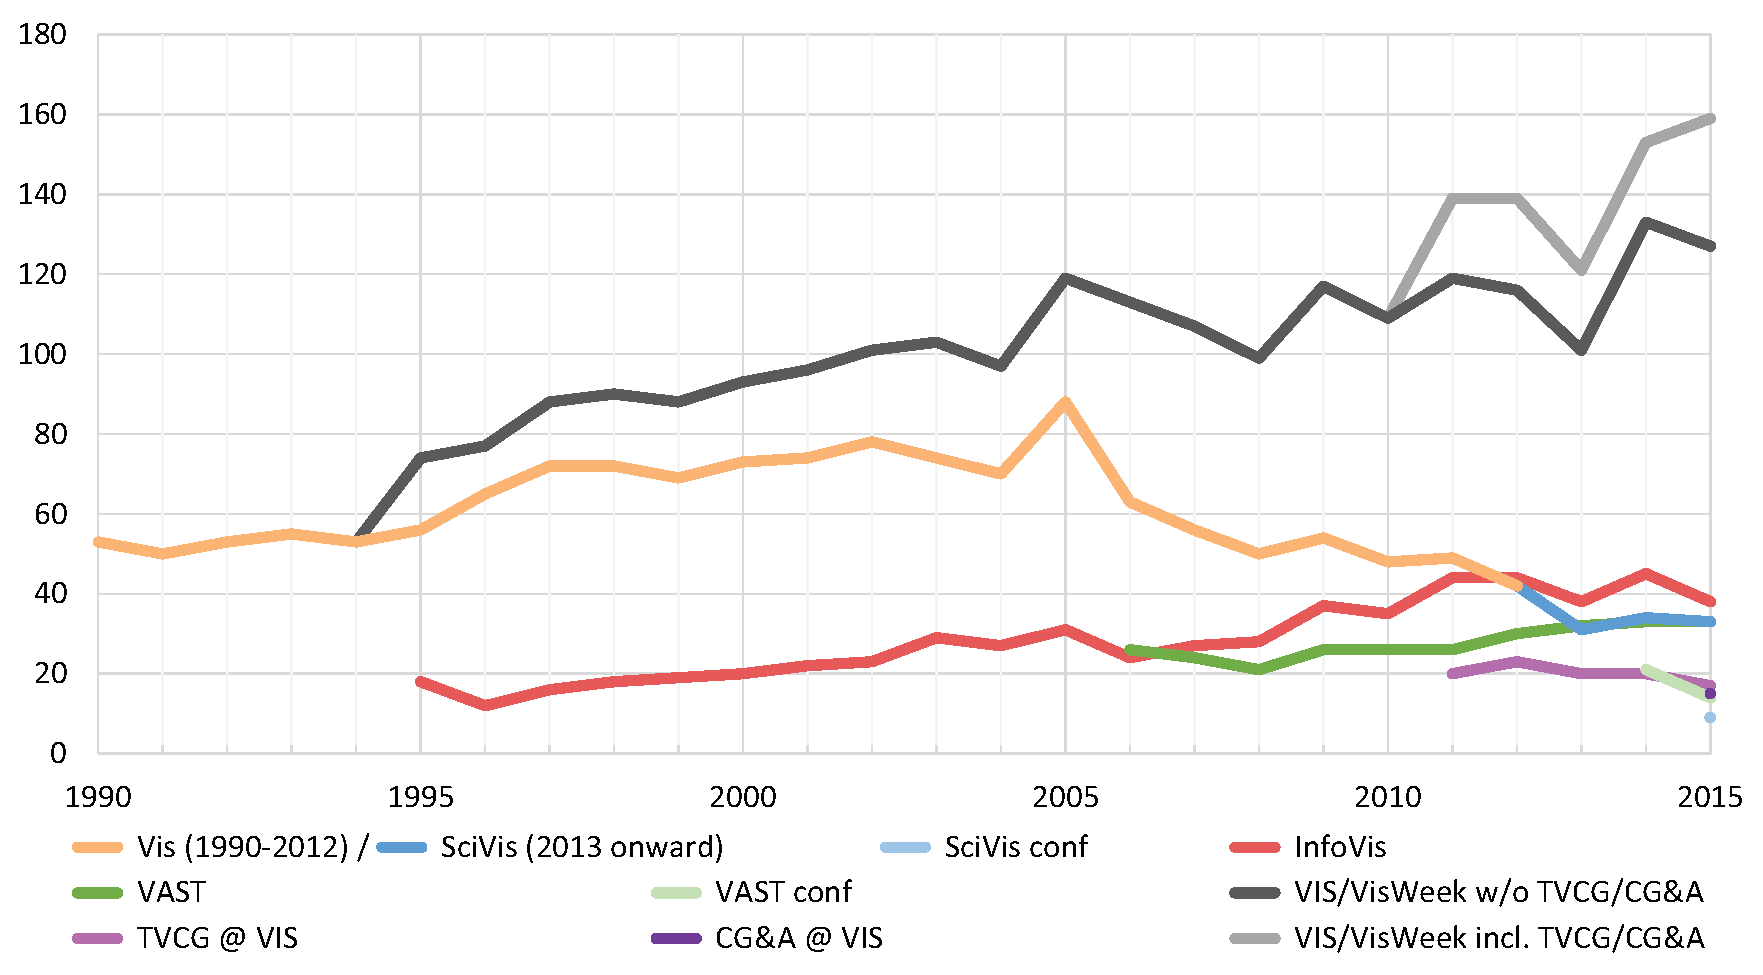
\includegraphics[width=\columnwidth]{paper-count-w-2015-new}
 \caption{A visualization of the data from \autoref{tab:vis_papers}. The image is from \cite{Isenberg:2017:VMC} and is in the public domain.}
 \label{fig:sample}
\end{figure}

\subsubsection{Ejector Seat Reservation}

Duis autem~\cite{Lorensen:1987:MCA}\footnote{The algorithm behind
Marching Cubes \cite{Lorensen:1987:MCA} had already been
described by Wyvill et al. \cite{Wyvill:1986:DSS} a year
earlier.} vel eum iriure dolor in hendrerit
in vulputate velit esse molestie consequat,\footnote{Footnotes
appear at the bottom of the column.} vel illum dolore eu
feugiat nulla facilisis at vero eros et accumsan et iusto odio
dignissim qui blandit praesent luptatum zzril delenit augue duis
dolore te feugait nulla facilisi. Lorem ipsum dolor sit amet,
consectetuer adipiscing elit, sed diam nonummy nibh euismod tincidunt
ut laoreet dolore magna aliquam erat volutpat.


\paragraph{Confirmed Ejector Seat Reservation}

Ut wisi enim ad minim veniam, quis nostrud exerci tation ullamcorper
suscipit lobortis nisl ut aliquip ex ea commodo
consequat~\cite{Nielson:1991:TAD}. Duis autem vel eum iriure dolor in
hendrerit in vulputate velit esse molestie consequat, vel illum dolore
eu feugiat nulla facilisis at vero eros et accumsan et iusto odio
dignissim qui blandit praesent luptatum zzril delenit augue duis
dolore te feugait nulla facilisi.

\paragraph{Rejected Ejector Seat Reservation}

Ut wisi enim ad minim veniam, quis nostrud exerci tation ullamcorper
suscipit lobortis nisl ut aliquip ex ea commodo consequat. Duis autem
vel eum iriure dolor in hendrerit in vulputate velit esse molestie


\section{Conclusion}

Lorem ipsum dolor sit amet, consetetur sadipscing elitr, sed diam
nonumy eirmod tempor invidunt ut labore et dolore magna aliquyam erat,
sed diam voluptua. At vero eos et accusam et justo duo dolores et ea
rebum. Stet clita kasd gubergren, no sea takimata sanctus est Lorem
ipsum dolor sit amet. Lorem ipsum dolor sit amet, consetetur
sadipscing elitr, sed diam nonumy eirmod tempor invidunt ut labore et
dolore magna aliquyam erat, sed diam voluptua. At vero eos et accusam
et justo duo dolores et ea rebum. Stet clita kasd gubergren, no sea
takimata sanctus est Lorem ipsum dolor sit amet. Lorem ipsum dolor sit
amet, consetetur sadipscing elitr, sed diam nonumy eirmod tempor
invidunt ut labore et dolore magna aliquyam erat, sed diam
voluptua. At vero eos et accusam et justo duo dolores et ea
rebum.


%% if specified like this the section will be committed in review mode
\acknowledgments{
The authors wish to thank A, B, C. This work was supported in part by
a grant from XYZ.}

%\bibliographystyle{abbrv}
\bibliographystyle{abbrv-doi}
%\bibliographystyle{abbrv-doi-narrow}
%\bibliographystyle{abbrv-doi-hyperref}
%\bibliographystyle{abbrv-doi-hyperref-narrow}

\bibliography{template}
\end{document}

